\documentclass[letterpaper,12pt,fleqn]{article}
\usepackage{matharticle}
\usepackage{siunitx}
\usepackage{pgfplots}
\pgfplotsset{compat=1.14}
\pagestyle{plain}
\begin{document}

\begin{center}
\Large Math-1003b Practice Final Exam
\end{center}

\vspace{1in}

\begin{enumerate}
\item Simplify the following expression:
  \[\left(\frac{x+3}{x^2-5x+6}\right)\left(\frac{4x-8}{x^2-9}\right)\]

\item Simplify the following expression:
  \[\frac{5}{2x}-\frac{3}{x+3}\]

\item A car completes in a NASCAR race on an oval track that measures
  $\SI{2}{miles}$ around. On the first lap the car is stuck in the pack, but
  breaks free on the second lap. The driver notices that the car is going
  $\SI{25}{mph}$ faster on the second lap. The car's timer measures that the
  car's second lap is $\SI{14.4}{seconds}$ ($\frac{1}{250}$ of an hour)
  faster than the first lap. What was the car's speed during the second lap?

\item Let $f(x)=x^{-\frac{2}{3}}+\abs{x}-3$. Evaluate the function at
  $x=-27$.

\item Sketch (do not plot points) for the following functions:
  \begin{enumerate}
  \item $f(x)=x^3$.

    \begin{tikzpicture}
      \draw (-3,0) -- (3,0);
      \draw (0,-3) -- (0,3);
    \end{tikzpicture}
\newpage
  \item $f(x)=\abs{x}$.

    \begin{tikzpicture}
      \draw (-3,0) -- (3,0);
      \draw (0,-3) -- (0,3);
    \end{tikzpicture}

  \end{enumerate}

\item Use the graph of $K(x)$ to answer the following questions:

  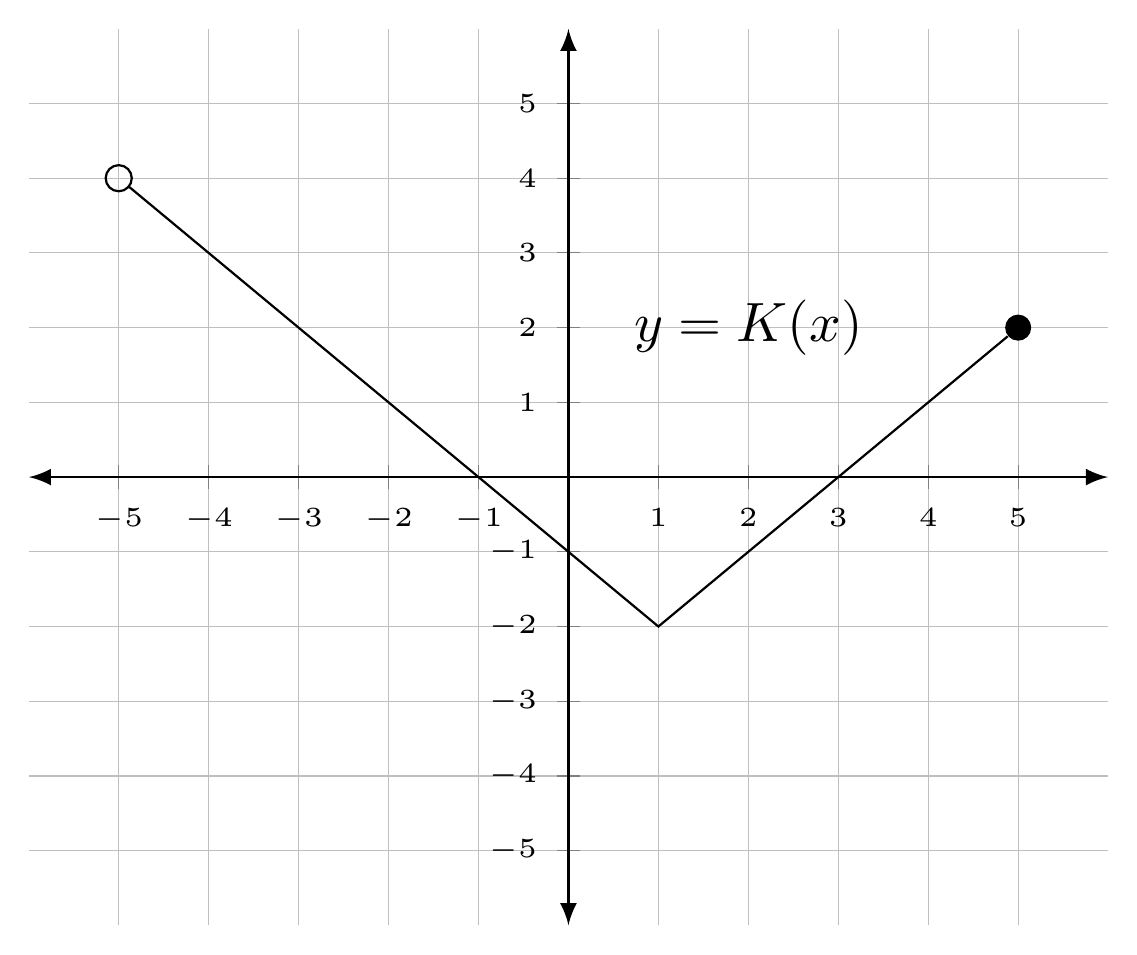
\begin{tikzpicture}[scale=2]
    \begin{axis}[
        xmin=-6,xmax=6,
        ymin=-6,ymax=6,
        grid=both,
        grid style={line width=.1pt, draw=gray!10},
        major grid style={line width=.2pt,draw=gray!50},
        axis lines=middle,
        axis line style={latex-latex},
        xtick={-5,-4,-3,-2,-1,0,1,2,3,4,5},
        ytick={-5,-4,-3,-2,-1,0,1,2,3,4,5},
        ticklabel style={font=\tiny},
      ]
      \node (a) [circle,draw,scale=0.5] at (-5,4) {};
      \node (b) [circle,fill,scale=0.5] at (5,2) {};
      \draw (a) to (1,-2) to (b);
      \node at (2,2) {$y=K(x)$};
    \end{axis}
  \end{tikzpicture}

  \begin{enumerate}
  \item What is $K(1)$?

  \item What is the y-intercept?

  \item For what values of $x$ is $K(x)=0$?

  \item What is the domain of $K$, in interval notation?

  \item What is the range of $K$, in interval notation?
  \end{enumerate}

\item Let $f(x)=x^2+1$ and $g(x)=x-3$. Perform the
  following operations:
  \begin{enumerate}
  \item $f+g$

  \item $fg$
    
  \item $\frac{f}{g}$
    
  \item $f\circ g$
    
  \item $g\circ f$

  \end{enumerate}

\item The area of a picture projected on a wall varies directly as the
  square of the distance from the projector to the wall. If a $\SI{5}{foot}$
  distance produces a picture with an area of $\SI{50}{square feet}$, then what
  is the area of a picture produced with the projection unit is moved to a
  distance $\SI{10}{feet}$ from the wall?

\item Solve the following inequalities. Your answers must be in interval
  notation:
  \begin{enumerate}
  \item $-3<2x-1\le3$

  \item $2x-1\le-3\ \mbox{or}\ 2x-1>3$

  \end{enumerate}

\item Solve the following inequalities. Your answers must be in interval
  notation:
  \begin{enumerate}
  \item $x^2-2x-8>0$

  \item $\frac{x+2}{x-4}\le0$

  \end{enumerate}

\item Solve for $x$:
  \begin{enumerate}
  \item $\abs{\frac{1}{3}x+2}-1=3$

  \item $\abs{\frac{1}{3}x+2}-1<3$
    
  \item $\abs{\frac{1}{3}x+2}-1\ge3$
  \end{enumerate}

\item Solve the following system of inequalities graphically. For full credit,
  determine and label the $x$ and $y$ intercepts for each line, sketch the
  two lines using the intercepts, and then select the correct region.
  \[\left\{\begin{array}{l} x+y<1 \\ 3x-2y\ge6 \end{array}\right.\]

  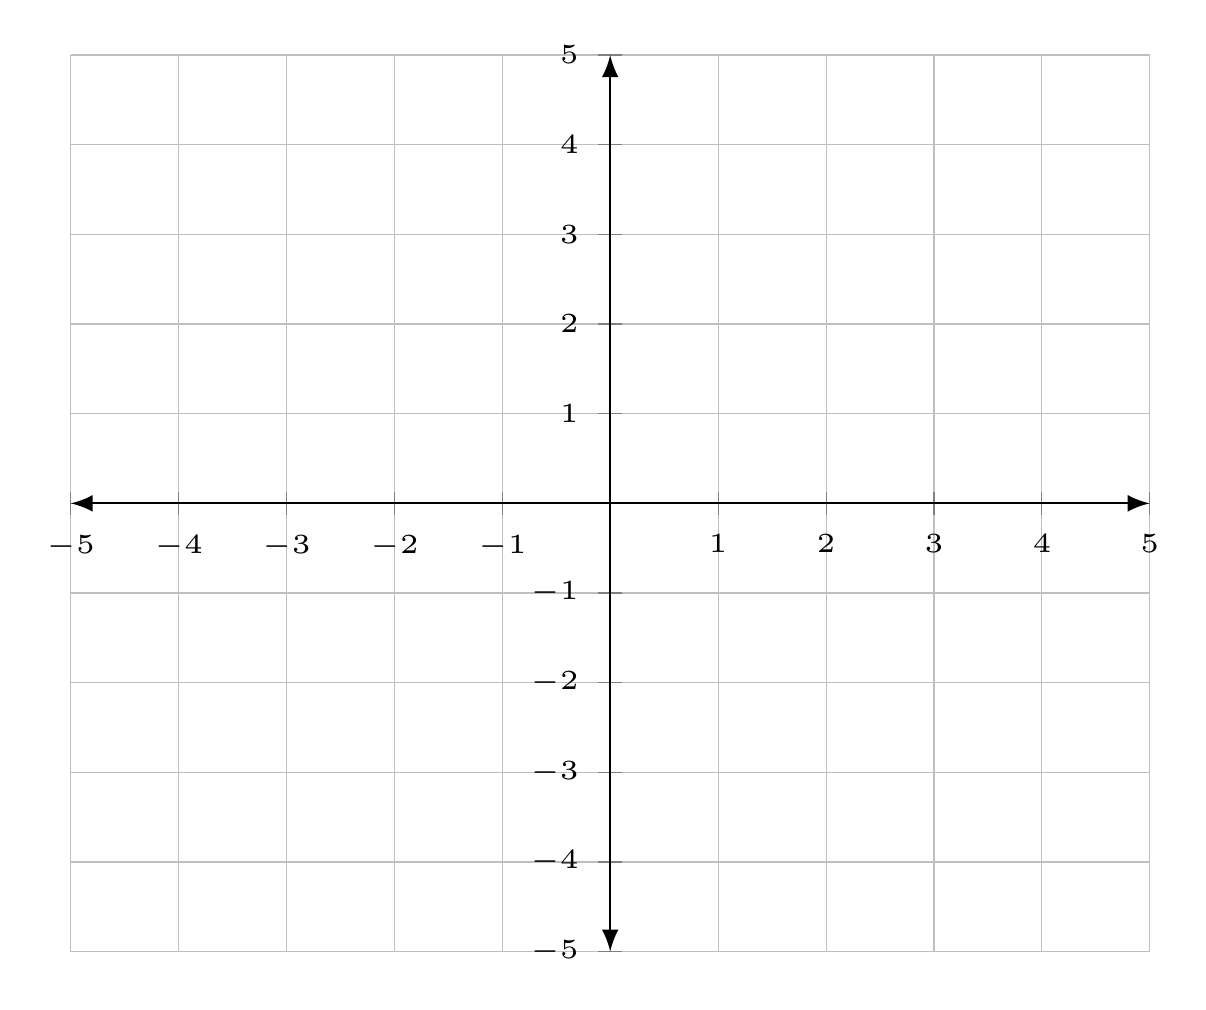
\begin{tikzpicture}[scale=2]
    \begin{axis}[
        xmin=-5,xmax=5,
        ymin=-5,ymax=5,
        grid=both,
        grid style={line width=.1pt, draw=gray!10},
        major grid style={line width=.2pt,draw=gray!50},
        axis lines=middle,
        axis line style={latex-latex},
        xtick={-5,-4,-3,-2,-1,0,1,2,3,4,5},
        ytick={-5,-4,-3,-2,-1,0,1,2,3,4,5},
        ticklabel style={font=\tiny},
      ]
    \end{axis}
  \end{tikzpicture}

\item Simplify (assume all variables are nonnegative):
  \[\left(\frac{54x^{-2}y^2}{2x^4y^{-4}}\right)^{\frac{1}{3}}\]

\item Evaluate each of the following. If not possible, say ``not a real
  number'':
  \begin{enumerate}
  \item $81^{\frac{5}{4}}$

  \item $-81^{\frac{5}{4}}$

  \item $(-81)^{\frac{5}{4}}$

  \item $-81^{-\frac{5}{4}}$

  \item $\sqrt[4]{81^5}$
  \end{enumerate}

\item Simplify:
  \[4b\sqrt{32b^3}-\sqrt{8b^5}\]
\newpage
\item Rationalize the denominators of the following:
  \begin{enumerate}
  \item \[\frac{xy}{\sqrt[3]{xy^2}}\]

  \item \[\frac{3}{\sqrt{x}-4}\]
  \end{enumerate}

\item Solve the following for $x$:
  \[\sqrt{3x+3}-1=x\]

  For problems $18-20$, consider the following general form of a parabola:
  \[y=2x^2+3x-5\]

\item Find the $x$-intercepts by completing the square.

\item Find the $x$-intercepts using the quadratic formula.

\item Convert to standard form by completing the square, note the $x$-intercepts from
  the previous problem, find the $y$ intercept and the vertex, and then sketch the graph.
  The intercepts and vertex MUST be labeled on your sketch for full credit!
\end{enumerate}

\end{document}
